\documentclass[main.tex]{subfiles}

\begin{document}

\section{模块设计}
\subsection{IFU}
\subsubsection{基本描述}
IFU完成程序计数器$PC$的维护、以及指令存储器$IM$的读取。
\paragraph{程序计数器$PC$的维护}
程序计数器$PC$的维护工作,即是在每次时钟信号$clk$出现上升沿时,根据输入的控制信号$NPCSel$,使用对应的方式生成新的PC值。支持为$beq$指令服务的相对跳转、为$j$指令服务的绝对跳转、为其他指令服务的$PC+4$三种模式。
\paragraph{指令存储器$IM$的读取}
程序计数器$PC$的值即是指令存储器$IM$的地址,该模块时刻读出$PC$指向$IM$中的值。

\subsubsection{模块接口}
\begin{center}
    \captionof{table}{IFU模块接口}
    \begin{tabular}[]{c c c l}
        \toprule
        信号名称 & 方向 & 位宽 & 描述 \\
        \midrule
        $clk$ & input & 1bit & 时钟信号。\\
        $reset$ & input & 1bit & \makecell[lt]{
            复位信号。\\
             0:复位。\\
             1:无效。
        } \\
        $NPCSel$ & input & 2bit & \makecell[lt]{
            新$PC$值生成方式选择的控制信号。\\
             00:使用$PC+4$模式生成\\
             01:使用相对跳转模式生成(服务$beq$等指令)\\
             10:使用绝对跳转模式生成(服务$j$等指令)
        } \\
        \midrule
        $BeqOffset$ & input & 16bit & 相对跳转位置。\\
        $JmpAddr$ & input & 26bit & 绝对跳转位置。 \\
        $Instr$ & output & 32bit & 32bit的$MIPS$指令。\\
        \bottomrule
    \end{tabular}
\end{center}

\subsubsection{功能定义}
\begin{center}
    \captionof{table}{IFU功能定义}
    \begin{tabular}{c c l}
        \toprule
        序号 & 功能名称 & 功能描述 \\
        \midrule
        1 & 复位 & $reset \land clk\uparrow \Rightarrow  PC \leftarrow 0x000003000$ \\
        2 & 取指令 & $Instr \leftarrow IM[PC] $ \\
        3 & 计算新的$PC$值 & \makecell[l]{ 
            $NPCSel == 0b00 \Rightarrow PC \leftarrow PC + 4 $ \\
            $NPCSel == 0b01 \Rightarrow PC \leftarrow PC + 4 + BeqOffset\ ||\ 0^2$ \\
            $NPCSel == 0b10 \Rightarrow PC \leftarrow (PC+4)_{31..28}\ ||\ JmpAddr\ ||\ 0^2 $ \\
        } \\
        \bottomrule
    \end{tabular}
\end{center}

\subsubsection{模块实现}
\begin{figure}[h]
\centering
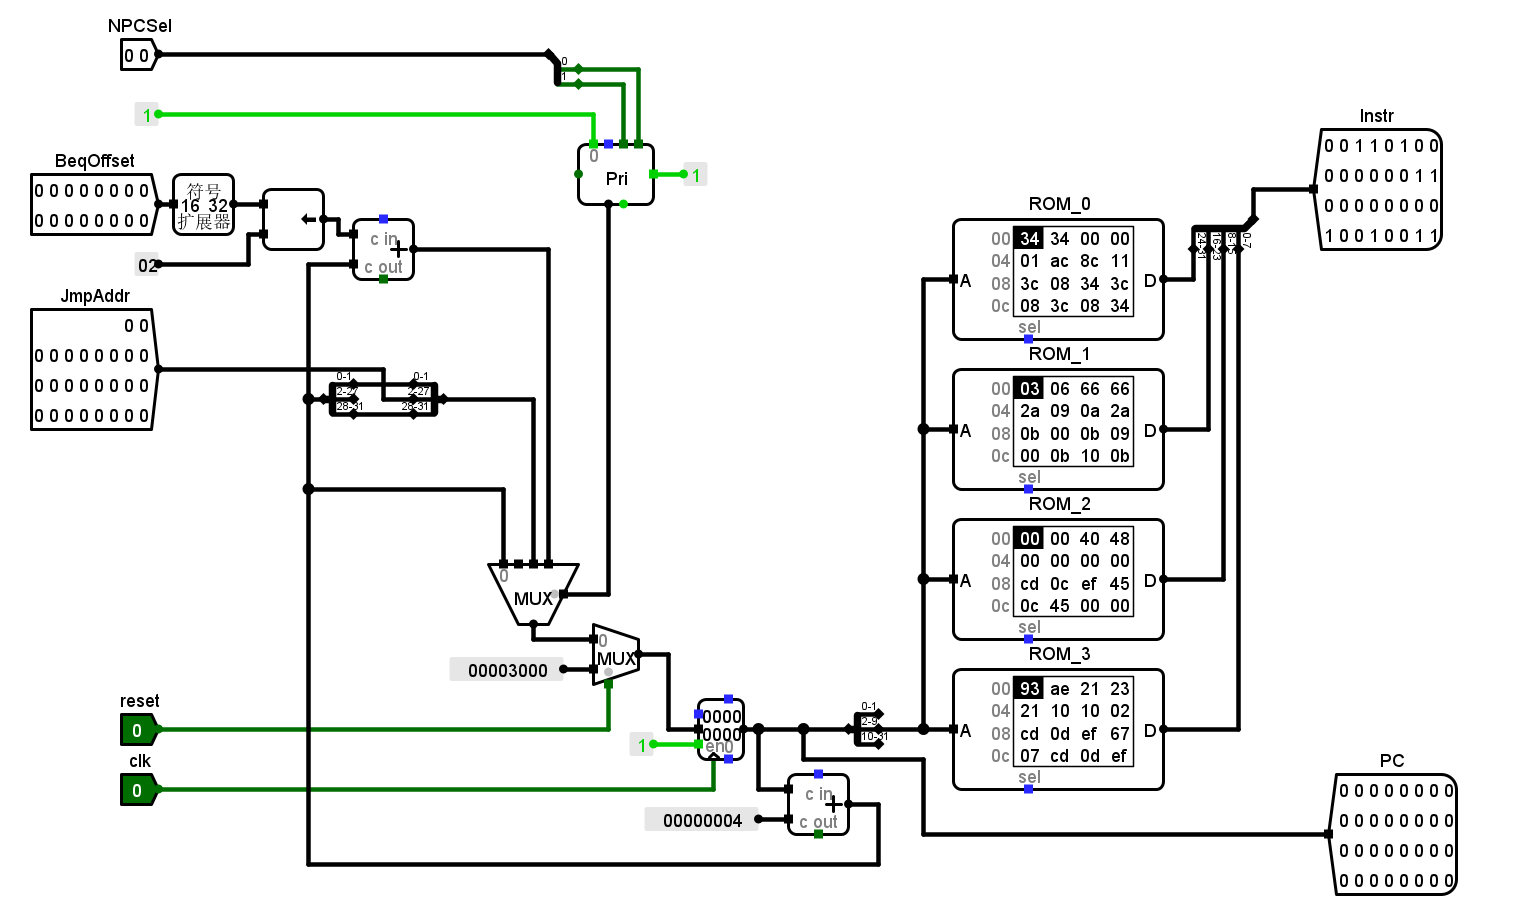
\includegraphics[width=\textwidth]{images/IFU-circuit.png}
\caption{IFU模块实现}
\end{figure}
IFU模块中,并行计算三种模式的新$PC$值,并通过$NPCSel$信号选择指定模式的新$PC$值,在$clk$出现上升沿时写入$PC$寄存器。

$PC$值作为指令存储器$IM$的地址,将对应数据输出到$Instr$。

\clearpage
\subsection{GPR}
\subsubsection{基本描述}
GPR为CPU寄存器组,完成$32$个32bit寄存器并行的两路读取和一路写入。
\paragraph{两路读取}
GPR根据输入的两寄存器编号$A_1$,$A_2$分别读取对应两寄存器数据$RD1$,$RD2$。
\paragraph{一路写入}
GPR根据输入的一寄存器编号$A_{wr}$将输入的数据$WD$存入对应的寄存器中。

\subsubsection{模块接口}
\begin{center}
    \captionof{table}{GPR模块接口}
    \begin{tabular}{c c c l}
        \toprule
        信号名称 & 方向 & 位宽 & 描述 \\
        \midrule
        $A_1$ & input & 5bit & 第一路读取寄存器编号 \\
        $A_2$ & input & 5bit & 第二路读取寄存器编号 \\
        $A_{wr}$ & input & 5bit & 写入寄存器编号 \\
        $D_{in}$ & input & 32bit & 写入的数据 \\
        $RD_1$ & output & 32bit & 第一路读取的数据 \\
        $RD_2$ & output & 32bit & 第二路读取的数据 \\
        \midrule
        $clk$ & input & 1bit & 时钟信号。\\
        $reset$ & input & 1bit & \makecell[lt]{
            复位信号。\\
             0:复位。\\
             1:无效。
        } \\
        $WE$ & input & 1bit & 高有效写允许信号 \\
        \bottomrule
    \end{tabular}
\end{center}

\subsubsection{功能定义}
\begin{center}
    \captionof{table}{GPR功能定义}
    \begin{tabular}{c c l}
        \toprule
        序号 & 功能名称 & 功能描述 \\
        \midrule
        1 & 复位 & $reset \land clk\uparrow \Rightarrow  Reg[i] = 0x00000000, i=0, 1, \dots 31 $ \\
        2 & 读取寄存器值 & $ RD_1 \leftarrow Reg[A_1], RD_2 \leftarrow Reg[A_2] $ \\
        3 & 写入寄存器值 & $A_{wr} \neq 0 \land WE \land clk\uparrow \Rightarrow Reg[A_{wr}] \leftarrow D_{in}$ \\
        \bottomrule
    \end{tabular}
\end{center}

\subsubsection{模块实现}
\begin{figure}[h]
\centering
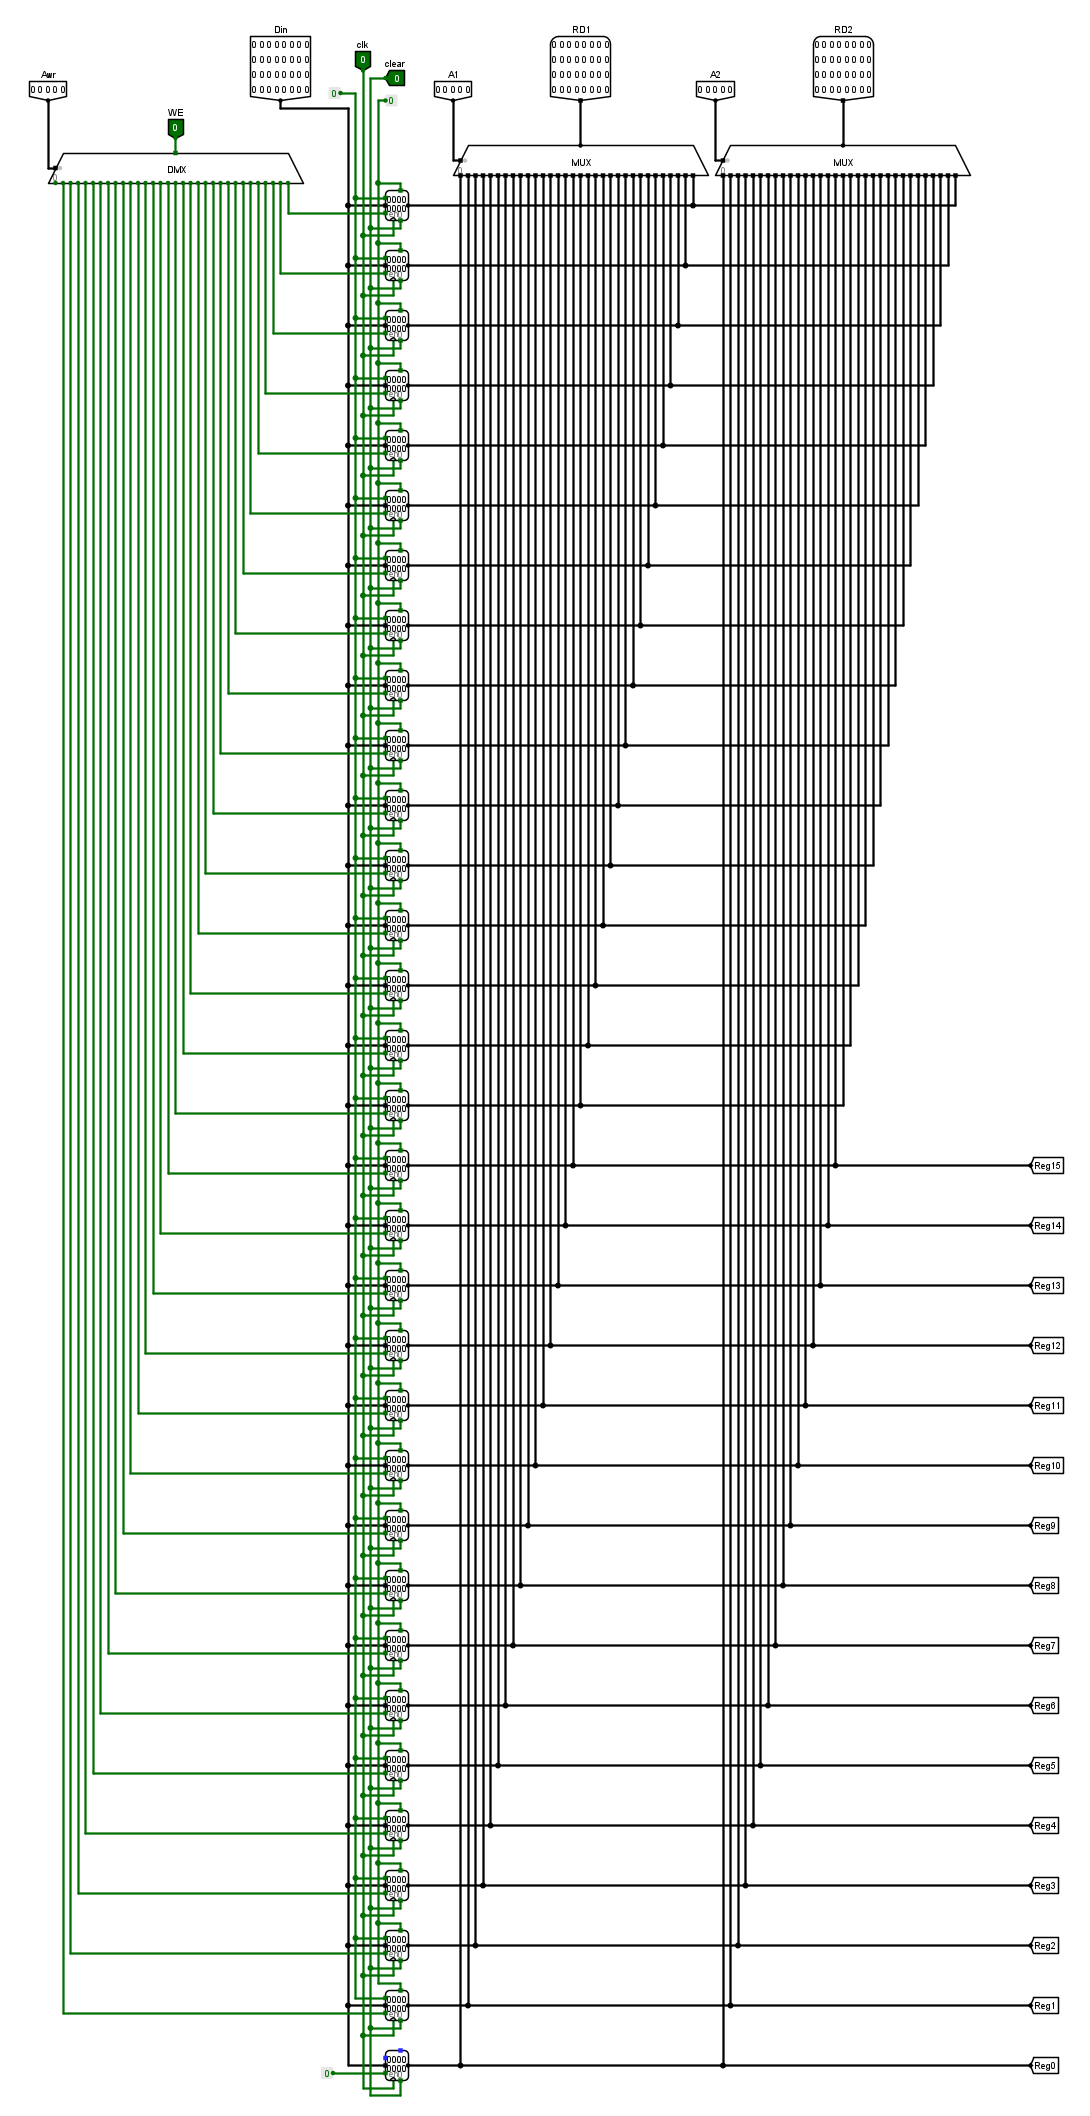
\includegraphics[width=0.8\textwidth]{images/GPR-circuit.png}
\caption{GPR模块实现}
\end{figure}
GPR模块由32个32bit寄存器、1个5-32的1bit解复用器(DMX)、2个32选1的32bit多路复用器(MUX)。

高有效写允许信号$WE$通过DMX分别连接到32个寄存器的使能端,给予对应寄存器写入使能。
32个寄存器的输出经过两个MUX分别将数据输出到$RD_1$、$RD_2$。

\clearpage
\subsection{ALU}
\subsubsection{基本描述}
ALU完成数据计算、数据比较、地址偏移量计算,具体为32bit的加、减、按位与、按位或四种运算功能。
\paragraph{加法运算}
ALU使用6组6bit并行加法器、组间提前进位运算器实现$6 \times 6$的36bit加法运算,并取其中低32位作为运算结果。
\paragraph{减法运算}
减法运算等价于第一运算数加上第二运算数的相反数。而根据补码的性质,一个数的相反数等于其自身取反加一。即$A-B = A+(-B) = A+\neg B+1$。
\paragraph{按位与运算}
按位与即是两运算数每位相与,用逻辑与门即可实现。
\paragraph{按位或运算}
按位与即是两运算数每位相或,用逻辑或门即可实现。

\subsubsection{模块接口}
\begin{center}
    \captionof{table}{ALU模块接口}
    \begin{tabular}{c c c l}
        \toprule
        信号名称 & 方向 & 位宽 & 描述 \\
        \midrule
        $ALUOp$ & input & 2bit & \makecell[lt]{
            $ALU$运算模式的控制信号。\\
             00:加法运算\\
             01:减法运算\\
             10:按位与运算 \\
             11:按位或运算
        } \\
        \midrule
        A & input & 32bit & 第一运算数。 \\
        B & input & 32bit & 第二运算数。 \\
        out & output & 32bit & 运算结果。 \\
        zero & output & 1bit & 结果是否为0。 \\
        \bottomrule
    \end{tabular}
\end{center}

\subsubsection{功能定义}
\begin{center}
    \captionof{table}{ALU功能定义}
    \begin{tabular}{c c l}
        \toprule
        序号 & 功能名称 & 功能描述 \\
        \midrule
        1 & 加法运算 & $ALUOp = 0b00 \Rightarrow out \leftarrow A+B$ \\
        2 & 减法运算 & $ALUOp = 0b01 \Rightarrow out \leftarrow A-B$ \\
        3 & 按位与运算 & $ALUOp = 0b10 \Rightarrow out \leftarrow A AND B$ \\
        4 & 按位或运算 & $ALUOp = 0b11 \Rightarrow out \leftarrow A OR B$ \\
        5 & 结果为零判断 & $zero \leftarrow \left( out = 0x00000000 \right) $ \\
        \bottomrule
    \end{tabular}
\end{center}

\subsubsection{模块实现}
\begin{figure}[h]
\centering
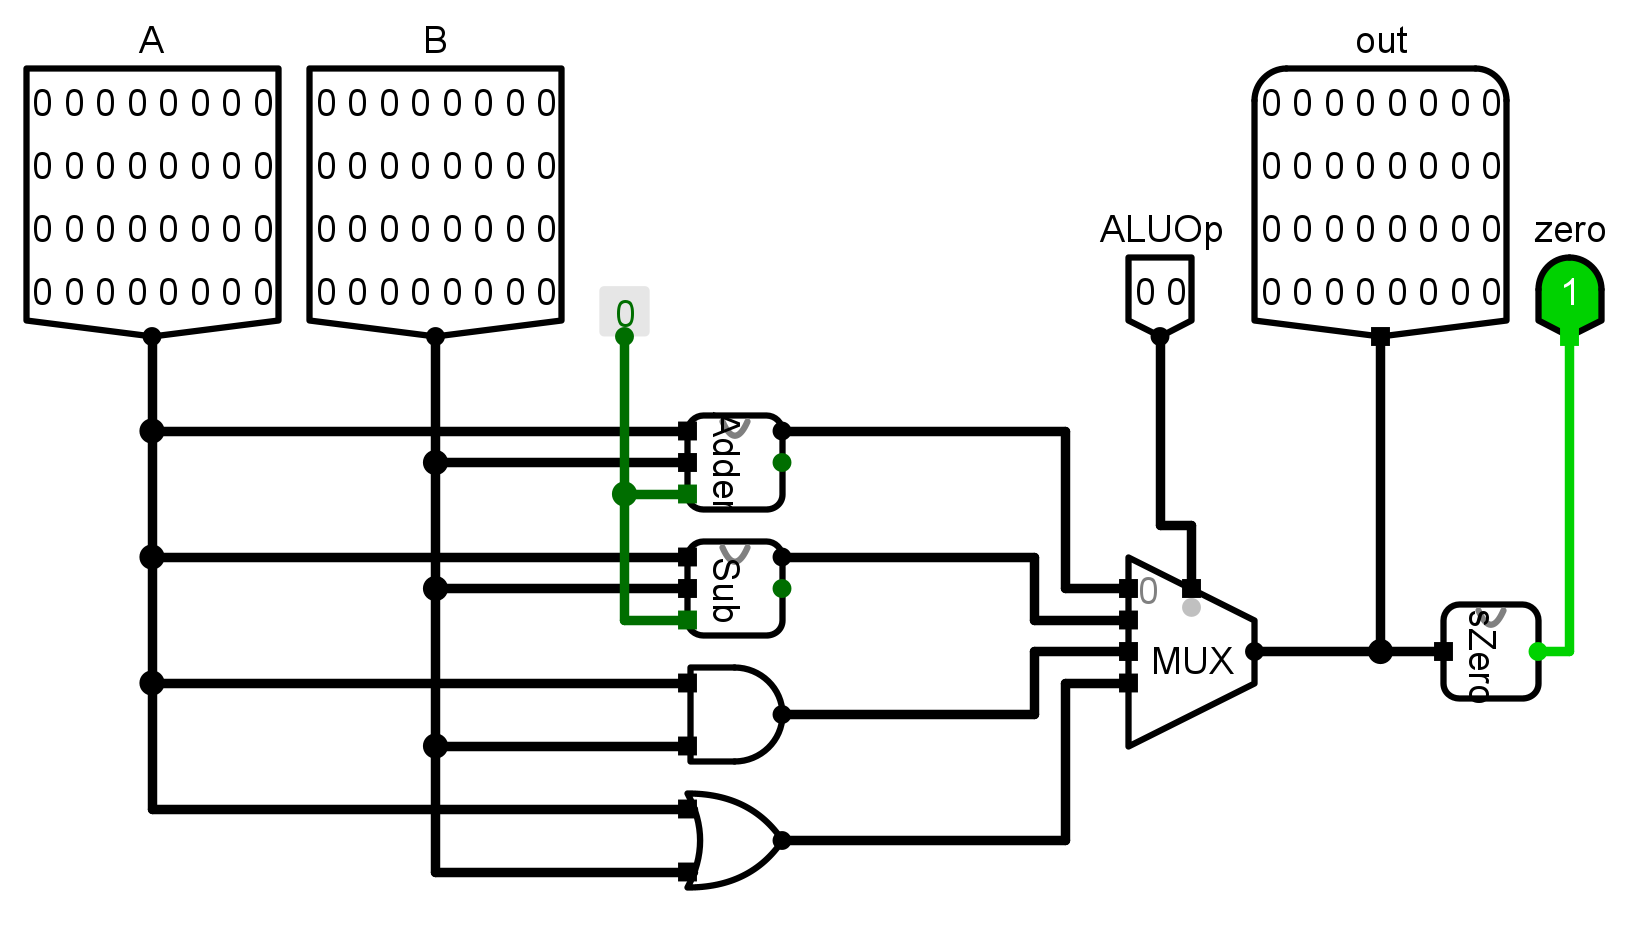
\includegraphics[width=\textwidth]{images/ALU-circuit.png}
\caption{ALU模块实现}
\end{figure}
$ALU$中并行计算两运算数的和、差、按位与结果、按位或结果。随后通过一个由$ALUOp$控制的多路复用器选择出对应的结果连接到$out$。$out$同时连接到零判断模块,结果输出到$zero$。

\paragraph{加法器($Adder$)}

\begin{figure}[H]
\centering
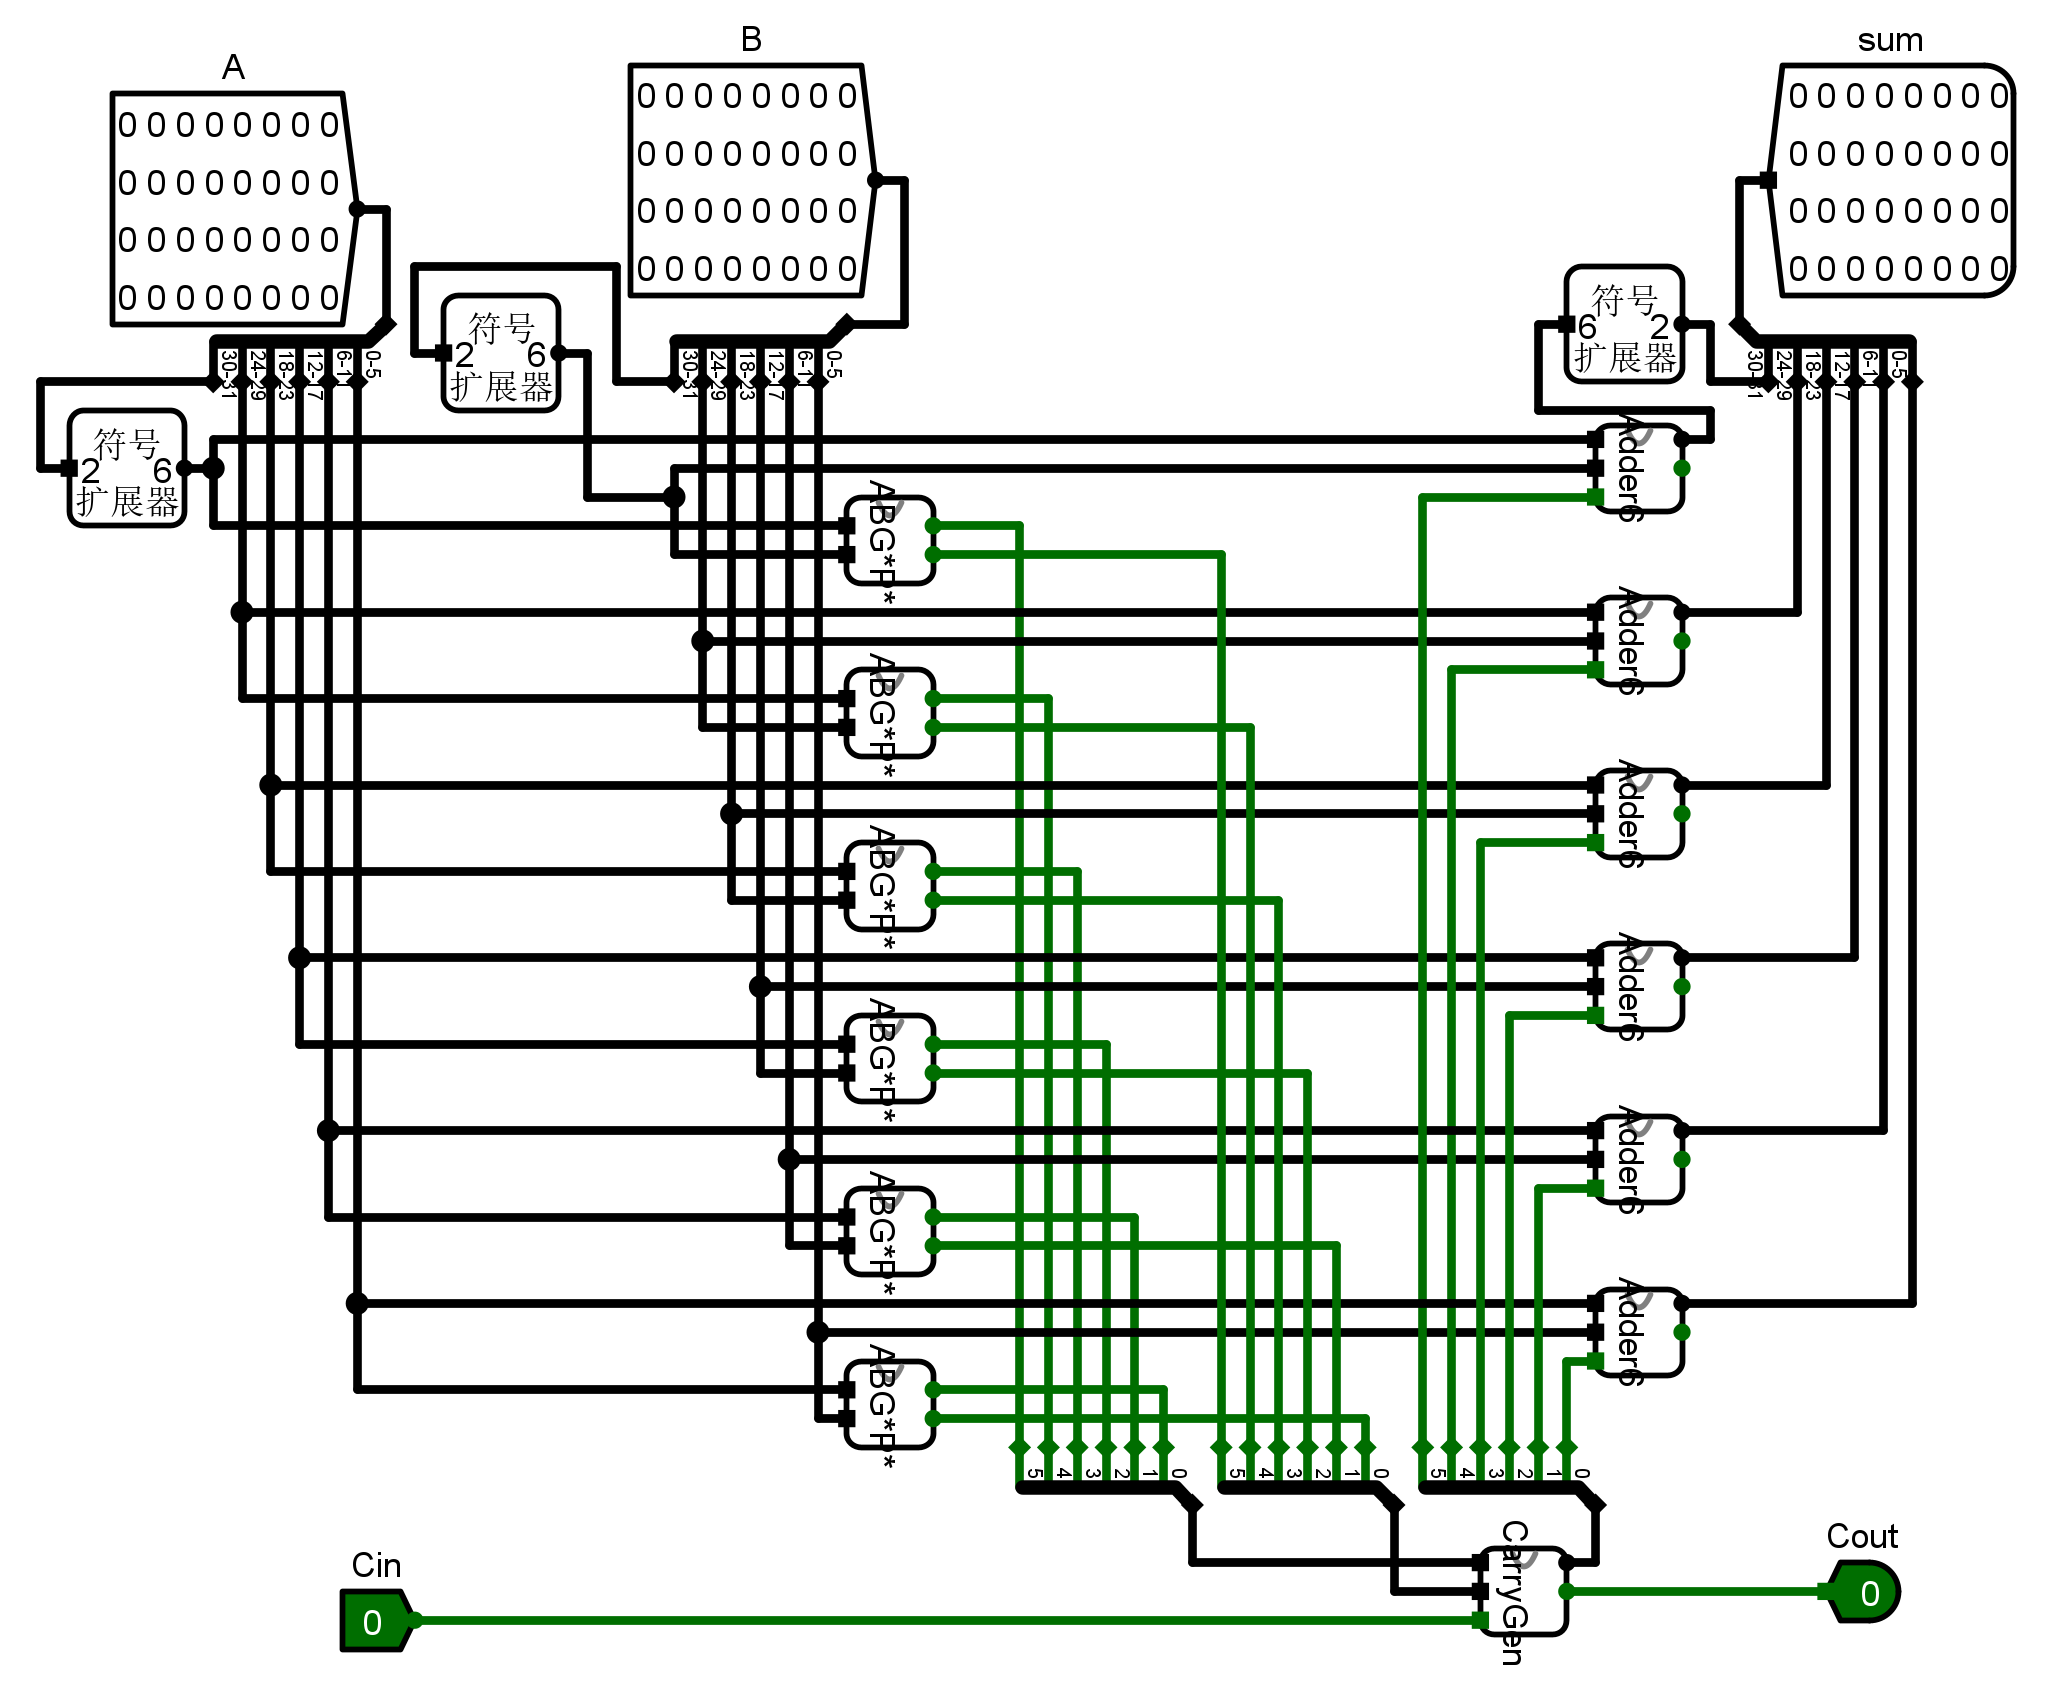
\includegraphics[width=\textwidth]{images/Adder-circuit.png}
\caption{加法器($Adder$)}
\end{figure}

加法器由6个6位加法器($Adder6$)、6个$G^*, P^*$生成器($ABG*P*$)和1个超前进位运算器($CarryGen$)组合而成。

每个6位加法器计算6位的和,超前进位运算器为它们提供进位输入,即可将6个6位加法器拼成36位并行加法器。
此外,输入对32位输入进行符号扩展到36位,输出则取36位结果中的低32位。



\subparagraph{6位加法器($Adder6$)} 

\begin{figure}[H]
\centering
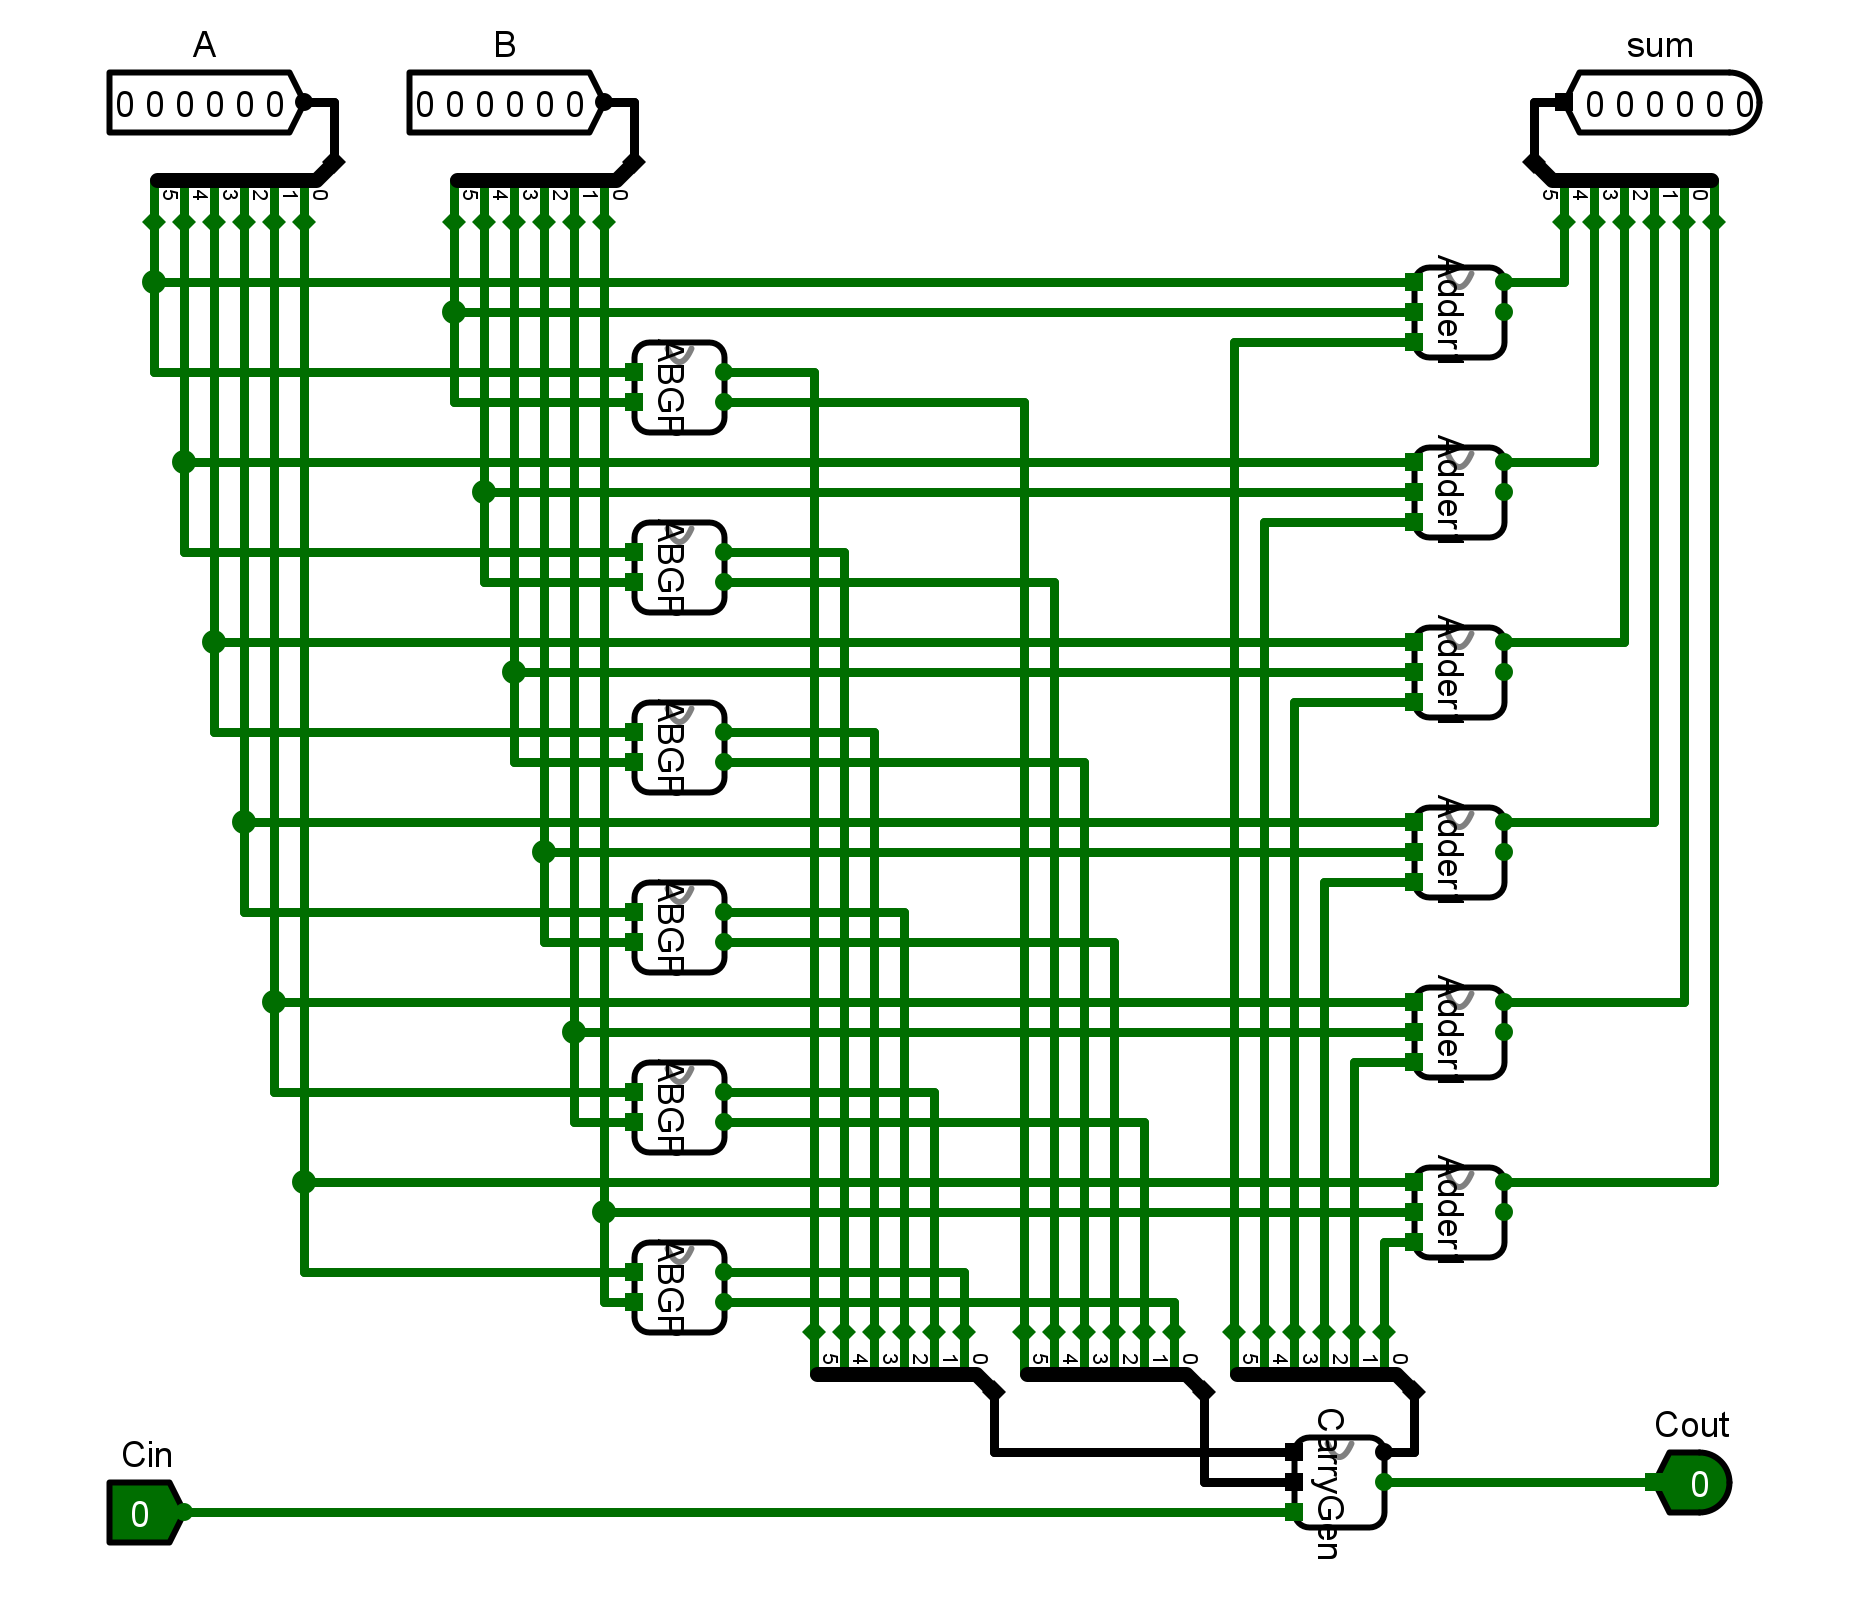
\includegraphics[width=\textwidth]{images/Adder6-circuit.png}
\caption{6位加法器($Adder6$)}
\end{figure}

6位并行加法器由6个全加器($Adder1$)、6个$G, P$生成器($ABGP$)和1个超前进位运算器($CarryGen$)组成。

每个全加器计算1位的和,超前进位运算器为它们提供进位输入。最终将6个1位全加器拼成6位加法器。



\subparagraph{超前进位运算器($CarryGen$)} 

\begin{figure}[H]
\centering
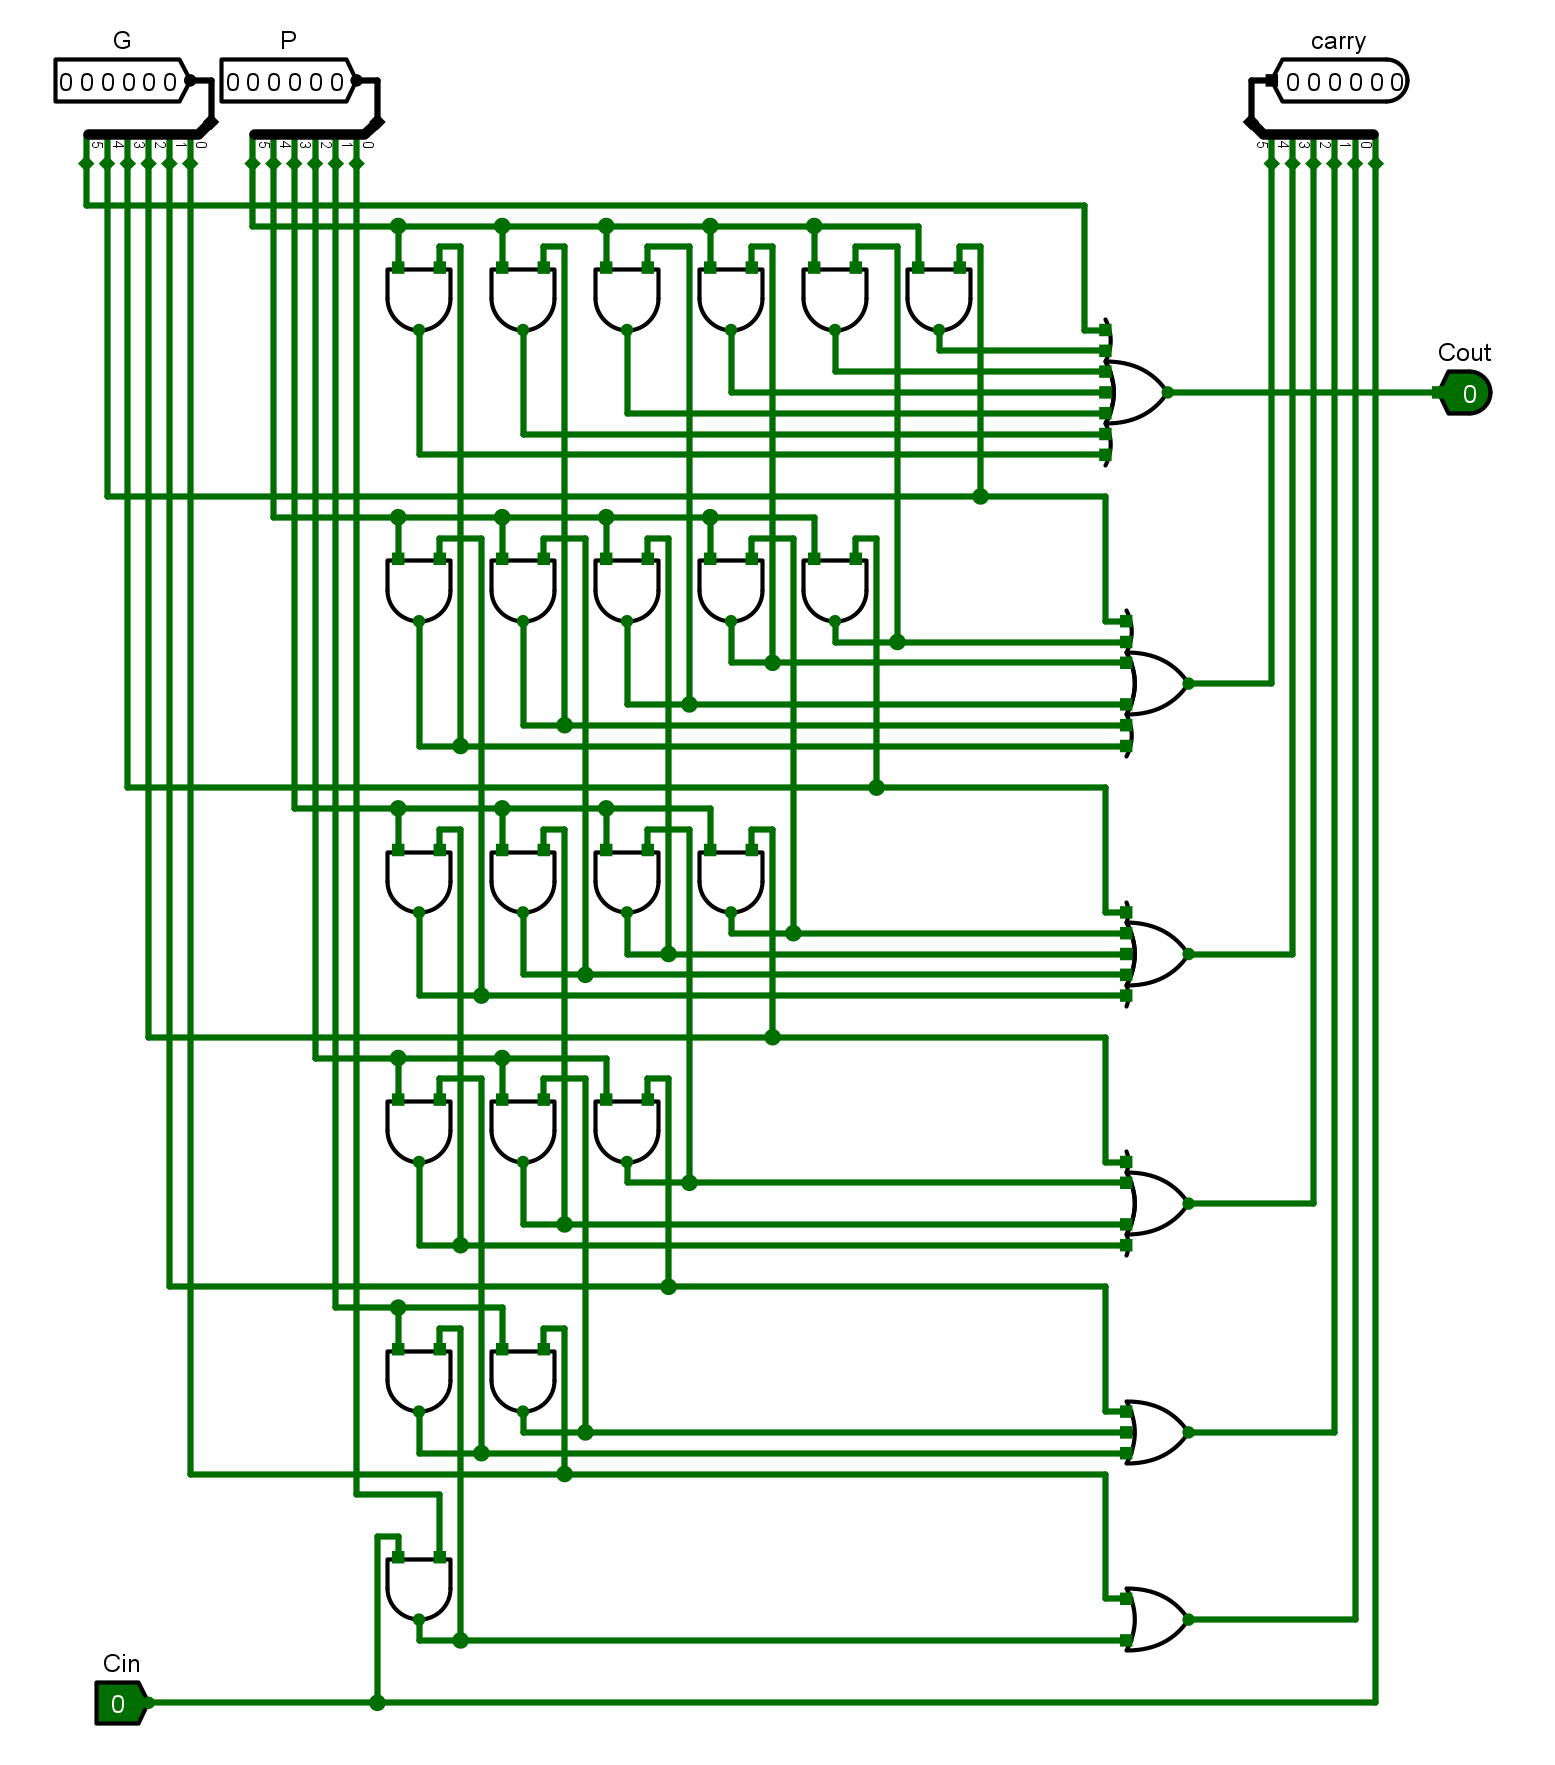
\includegraphics[width=\textwidth]{images/CarryGen-circuit.png}
\caption{超前进位运算器($CarryGen$)}
\end{figure}

超前进位运算器由逻辑与门、或门组成。它根据输入的6组$P, G$(或$P^*, G^*$)值计算出6组超前进位值。公式如下:

$$
\begin{array}{rcl}
C_1 &\leftarrow& G_0+P_0C_0 \\
C_2 &\leftarrow& G_1+P_1G_0+P_1P_0C_0 \\
C_3 &\leftarrow& G_2+P_2G_1+P_2P_1G_0+P_2P_1P_0C_0 \\
C_4 &\leftarrow& G_3+P_3G_2+P_3P_2G_1+P_3P_2P_1G_0+P_3P_2P_1P_0C_0 \\
C_5 &\leftarrow& G_3+P_3G_2+P_3P_2G_1+P_3P_2P_1G_0+P_3P_2P_1P_0C_0 \\
\end{array}
$$




\subparagraph{$P, G$生成器($ABPG$)}

\begin{figure}[H]
\centering
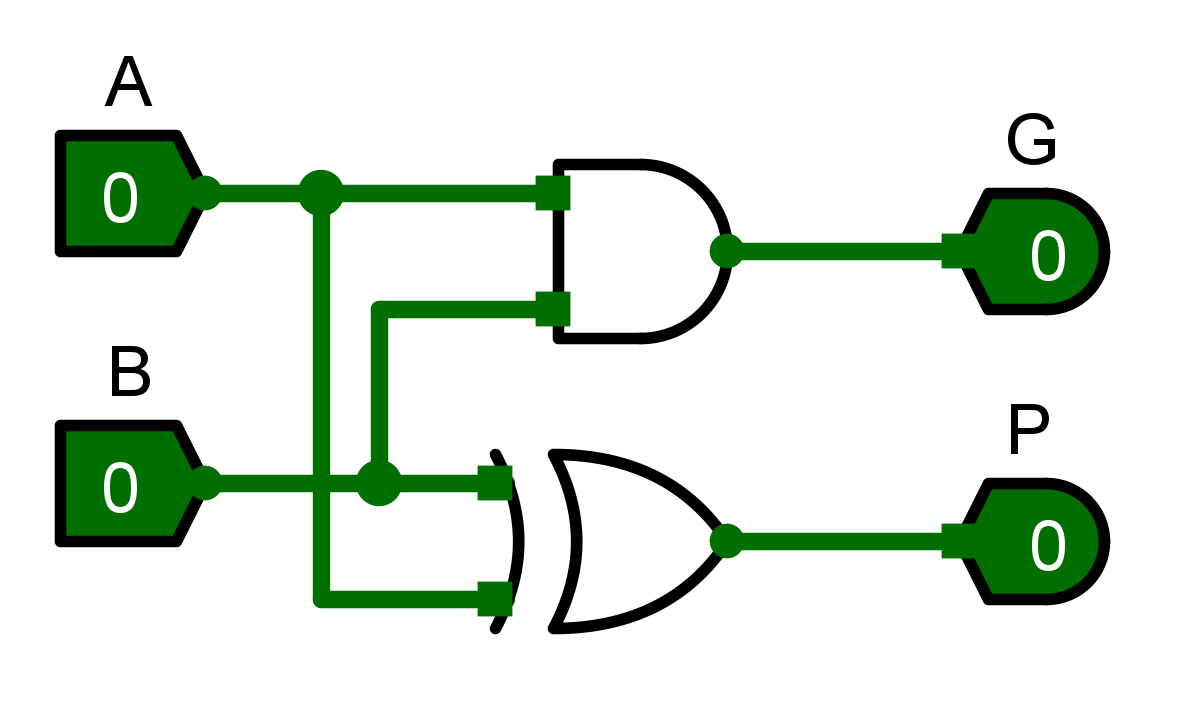
\includegraphics[width=0.6\textwidth]{images/ABGP-circuit.png}
\caption{$P, G$生成器($ABPG$)}
\end{figure}

$P, G$生成器由两加数$A, B$生成对应的$P, G$。使用一个与门和一个异或门,公式如下:
$$
\begin{array}{rcl}
G &\leftarrow& AB \\
P &\leftarrow& A \oplus B \\
\end{array}
$$

\subparagraph{$P^*, G^*$生成器($ABP*G*$)}

\begin{figure}[H]
\centering
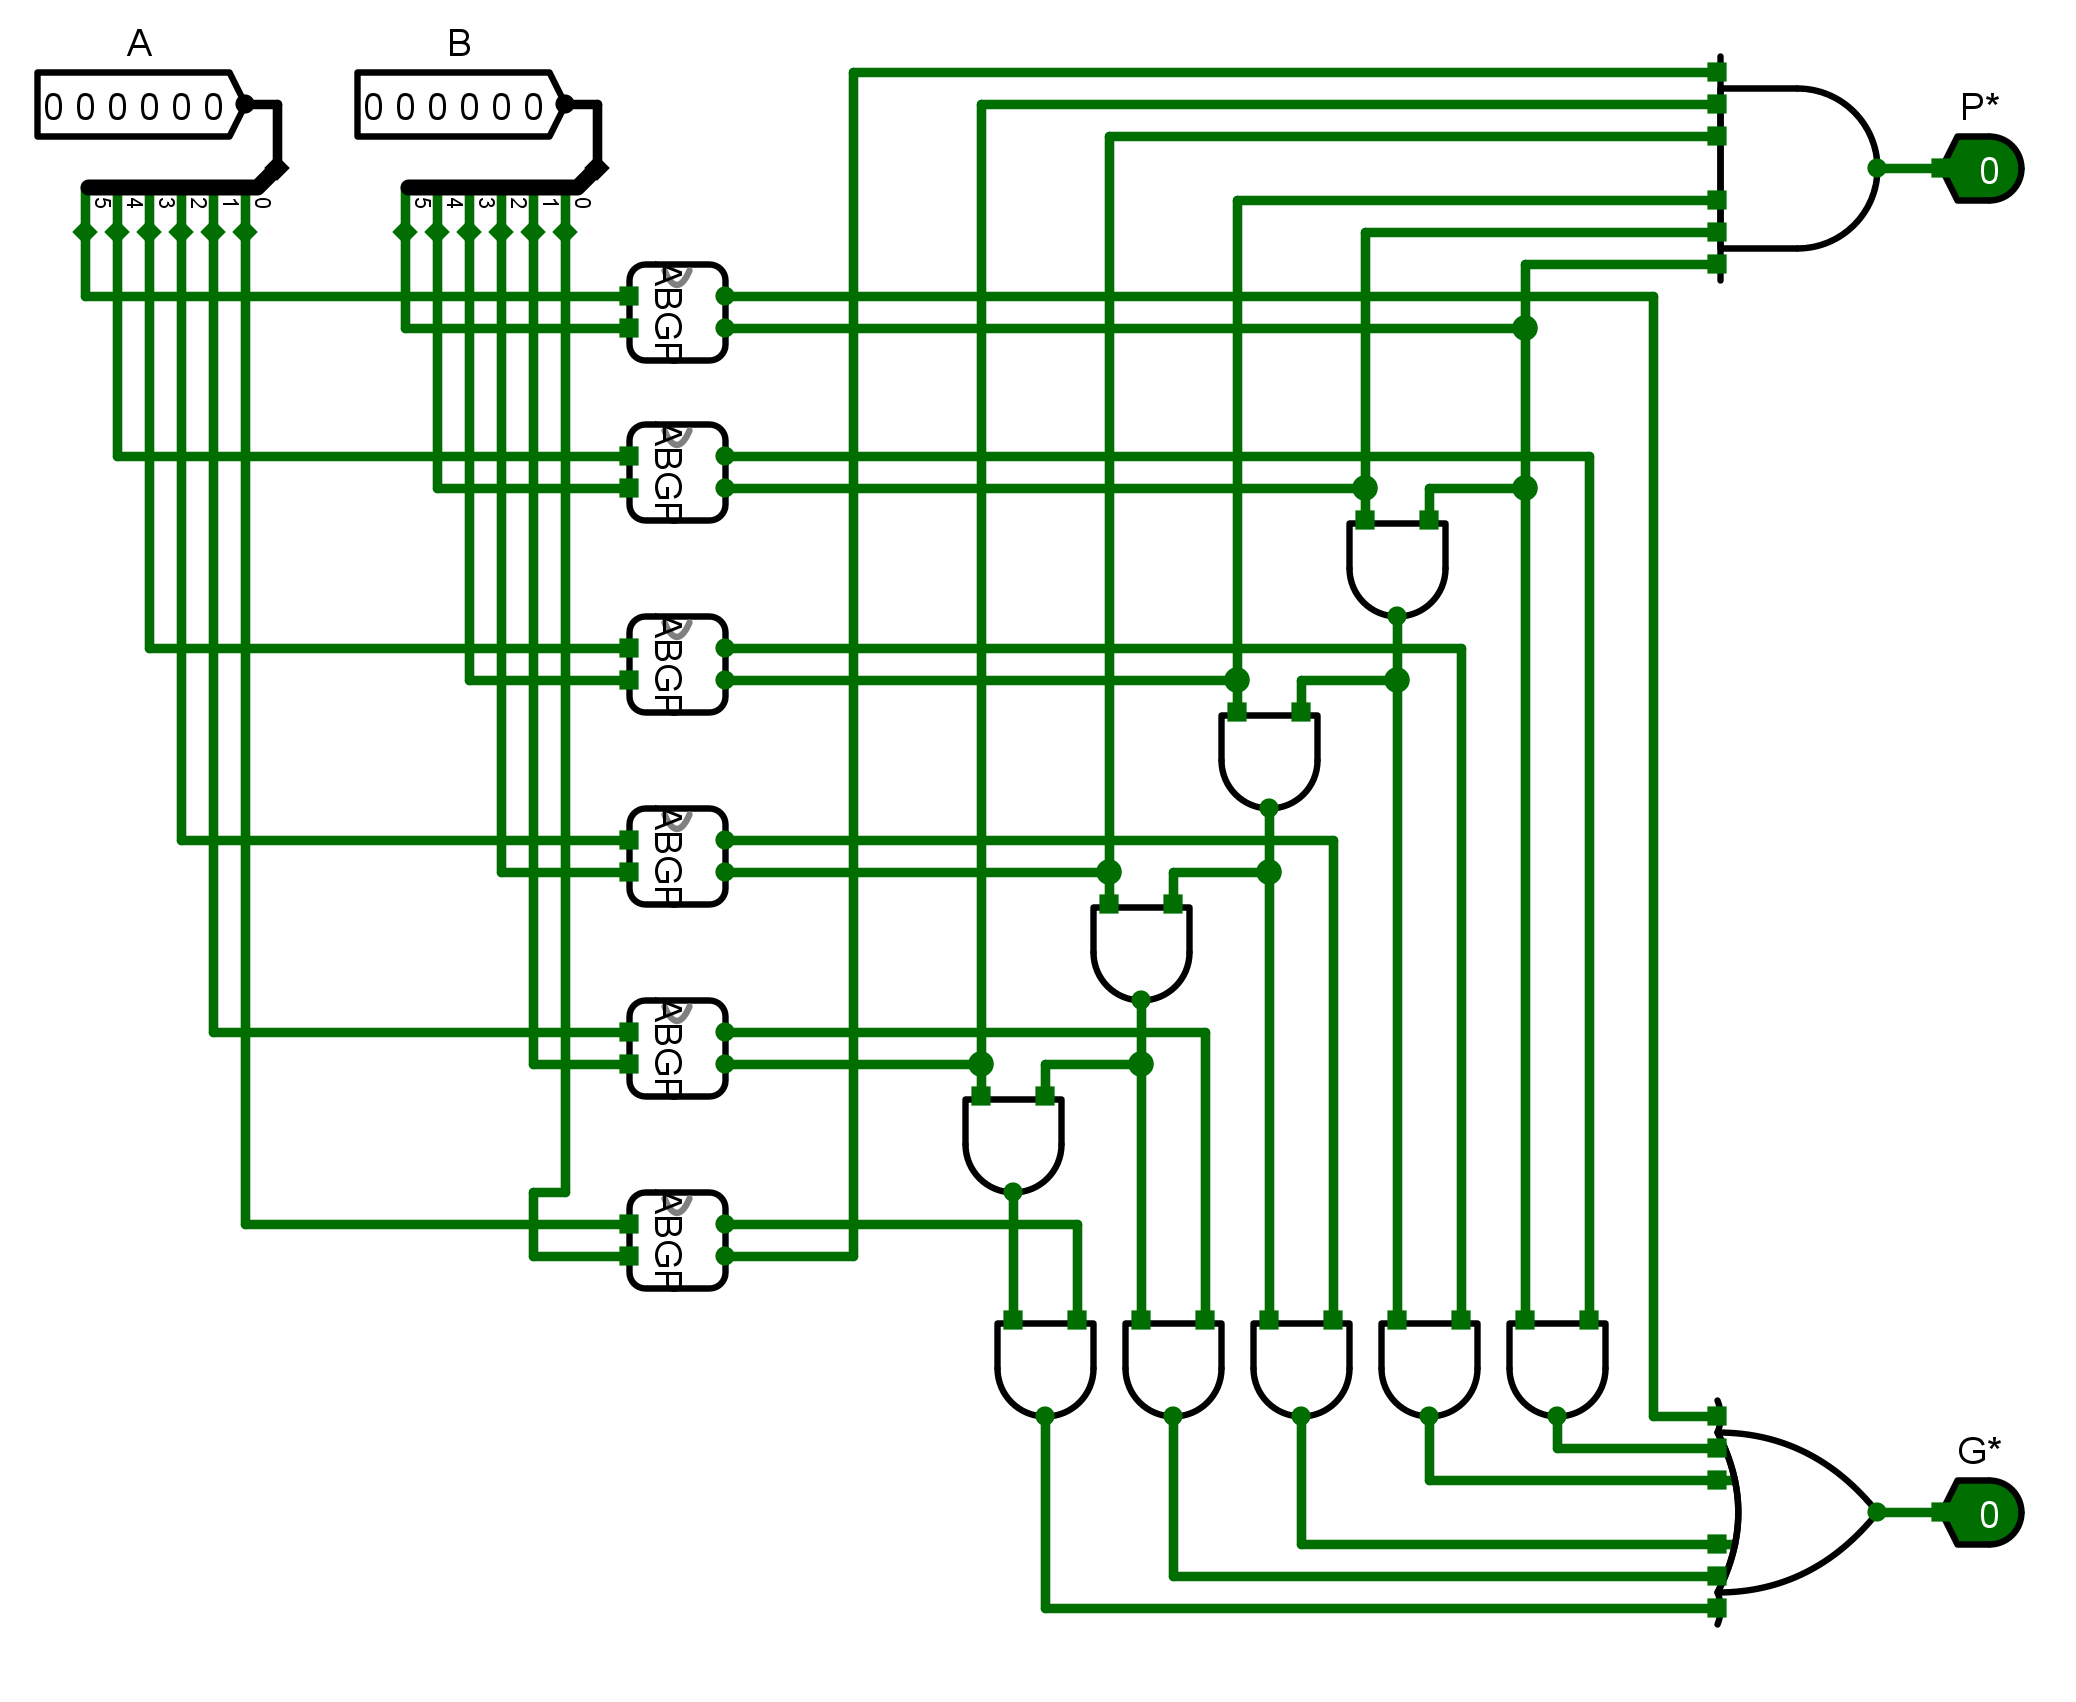
\includegraphics[width=\textwidth]{images/ABGxPx-circuit.png}
\caption{$P^*, G^*$生成器($ABP*G*$)}
\end{figure}

$P, G$生成器由两加数$A, B$生成对应的$P^*, G^*$。由六个$P, G$生成器($ABPG$)和数个逻辑与门、或门组成。

由两加数$A, B$先生成对应的$P, G$,再生成一组用于组间进位的$P^*, G^*$。公式如下:
$$
\begin{array}{rcl}
G_0^* &\leftarrow& G_5+P_5G_4+P_5P_4G_3+P_5P_4P_3G_2+P_5P_4P_3P_2G_1+P_5P_4P_3P_2P_1G_0 \\
P_5^* &\leftarrow& P_5P_4P_3P_2P_1P_0 \\
\end{array}
$$

\subparagraph{全加器($Adder1$)}

\begin{figure}[H]
\centering
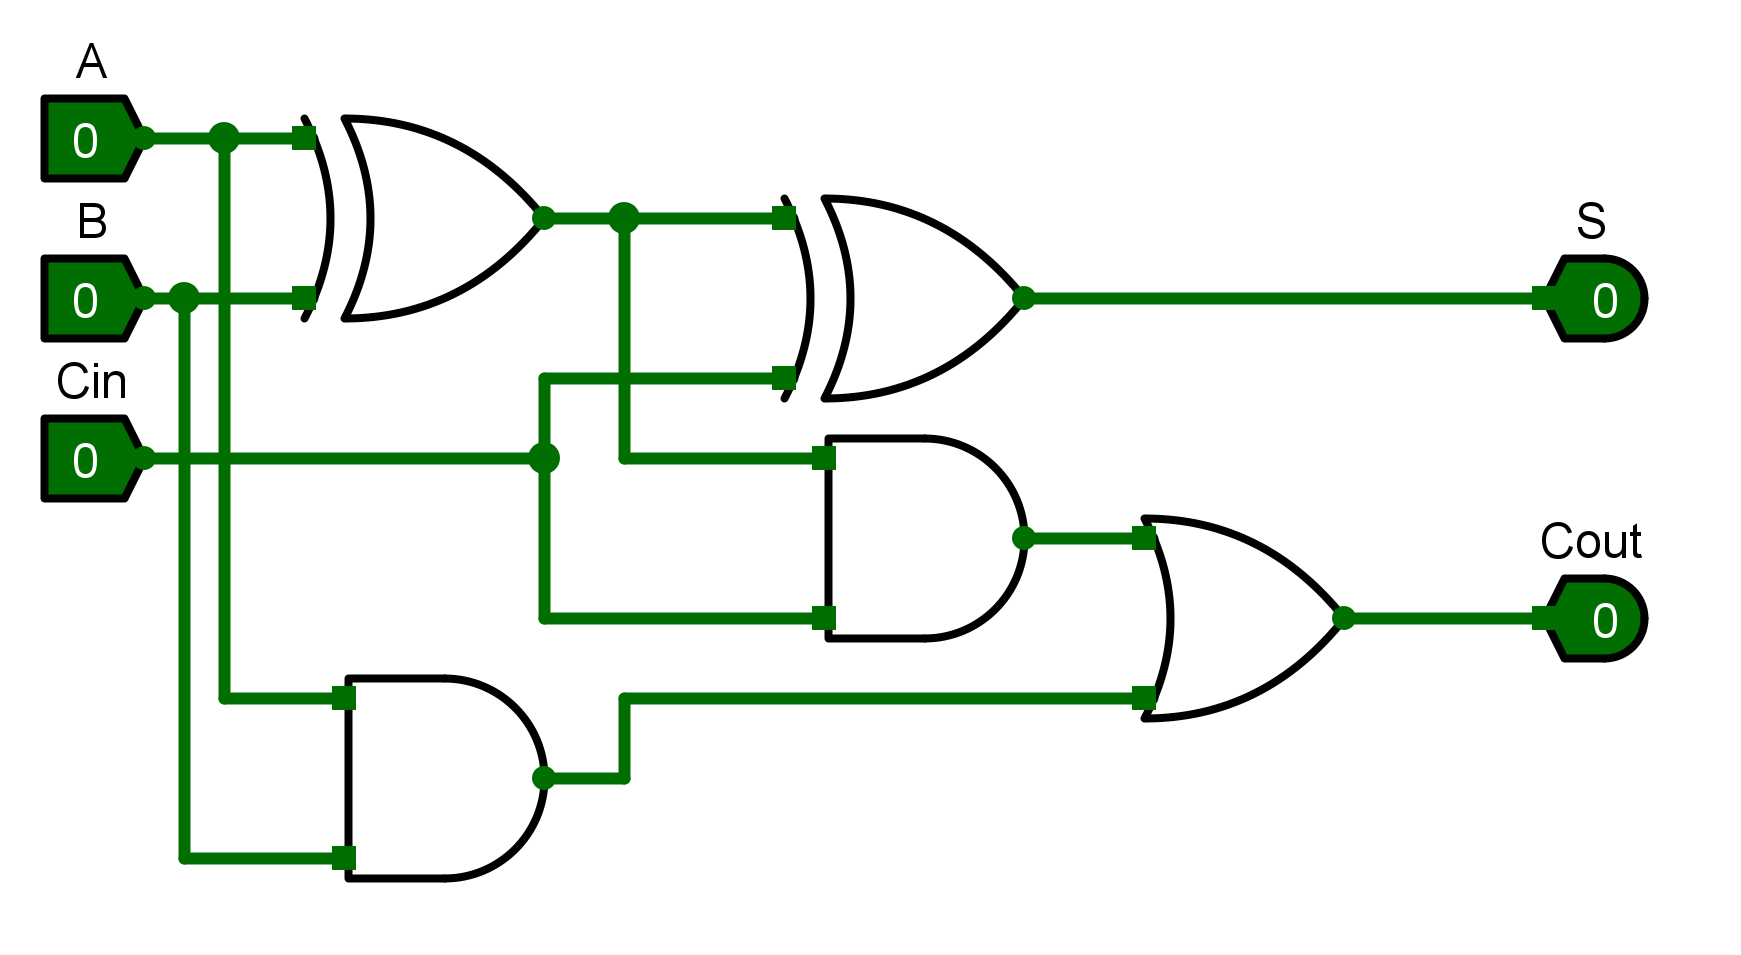
\includegraphics[width=0.6\textwidth]{images/Adder1-circuit.png}
\caption{全加器($Adder1$)}
\end{figure}

全加器可计算两个1位数的和,同时具有进位输入、进位输出。由逻辑与门、或门、异或门组成,公式如下:
$$
\begin{array}{rcl}
S &\leftarrow& A \oplus B \oplus C_{in} \\
C_{out} &\leftarrow& AB + C_{in}\left( A\oplus B\right) \\
\end{array}
$$

\paragraph{减法器($Subtractor$)}

\begin{figure}[H]
\centering
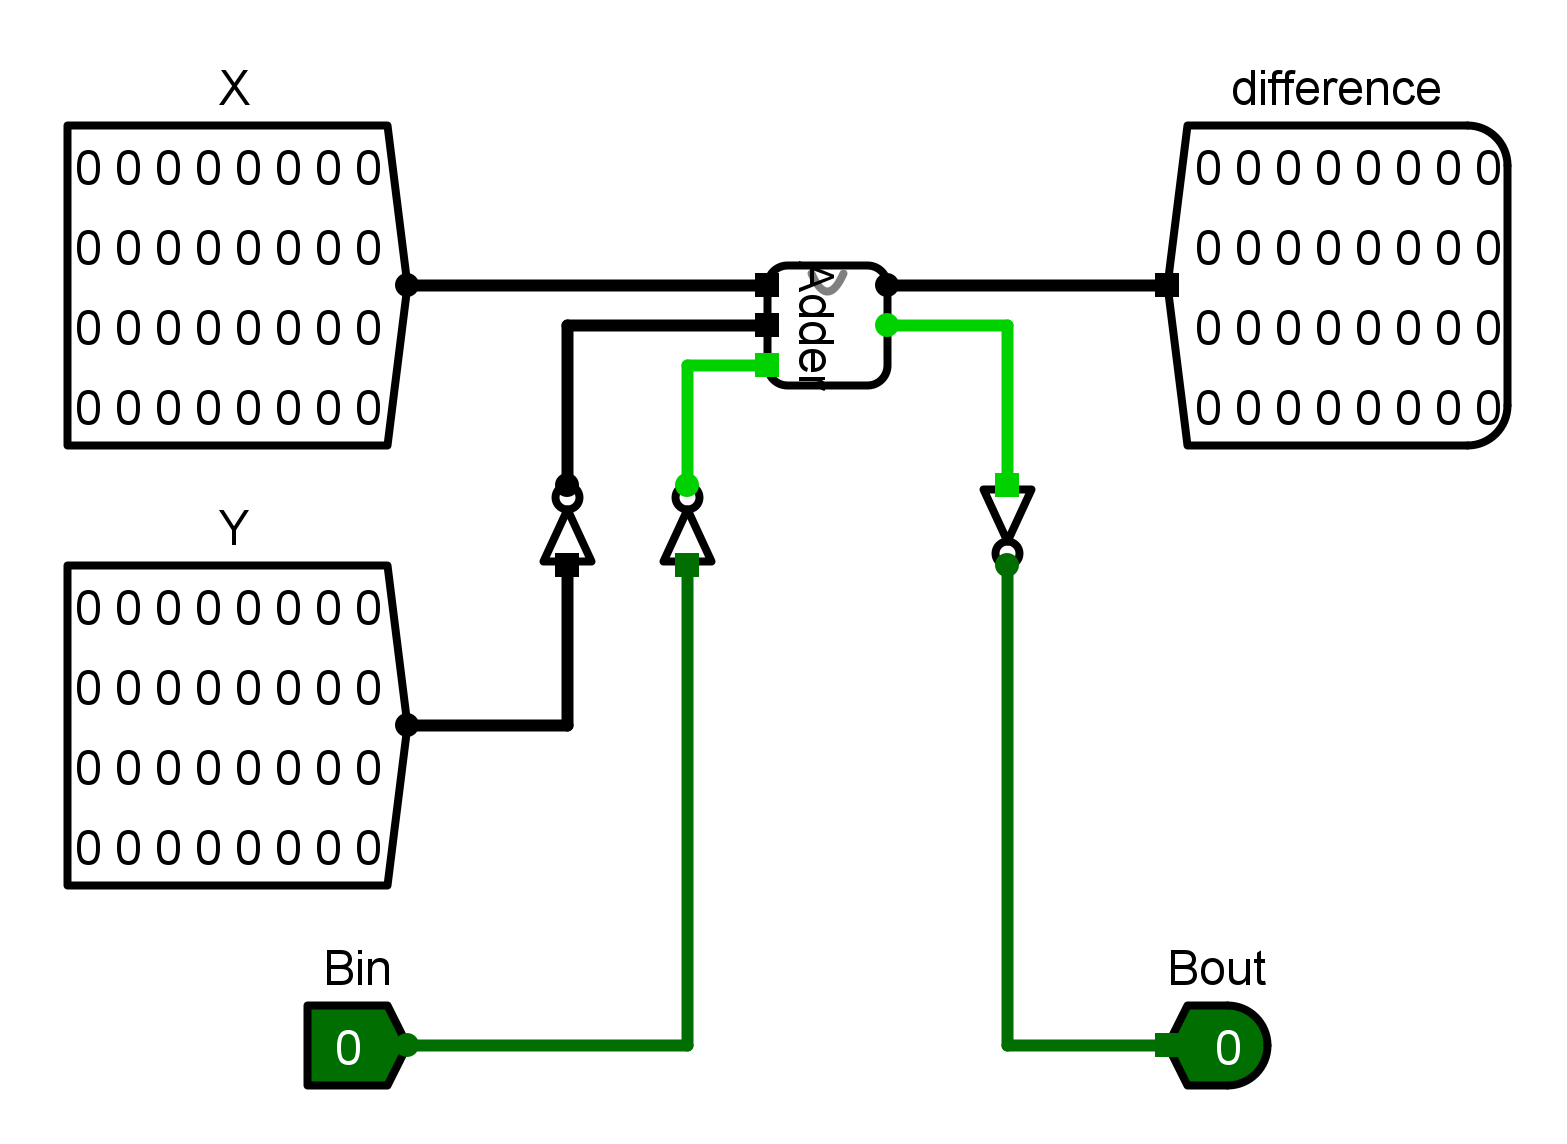
\includegraphics[width=0.6\textwidth]{images/Substractor-circuit.png}
\caption{减法器($Subtractor$)}
\end{figure}

借助补码的性质,减法运算由公式$A-B = A+(-B) = A+\neg B+1$转化为非运算和加法运算。而将借位输入取反作为加法器的进位输入就实现了$+1$的效果,再将加法器的进位输出取反即可得到借位输出。

因此减法器由1个加法器、1个32位非门、2个1位非门组成。

\paragraph{按位与和按位或}
按位与、按位或是将两操作数的每位对应求逻辑与、逻辑或。使用32位2输入的与门、或门即可实现。


\clearpage
\subsection{EXT}
\subsubsection{基本描述}
EXT完成从16位数据拓展到32位的三种拓展,并根据$ExtOp$指令选择对应的结果输出。三种拓展具体为零拓展、符号拓展、高位载入拓展。

\subsubsection{模块接口}
\begin{center}
    \captionof{table}{EXT模块接口}
    \begin{tabular}[]{c c c l}
        \toprule
        信号名称 & 方向 & 位宽 & 描述 \\
        \midrule
        $ExtOp$ & input & 2bit & \makecell[lt]{
            拓展模式选择的控制信号。\\
             00:输出零拓展 \\
             01:输出符号拓展 \\
             10:输出高位载入拓展 \\
        } \\
        \midrule
        $imm16$ & input & 16bit & 16位输入数据。\\
        $ext32$ & output & 32bit & 32位拓展结果。 \\
        \bottomrule
    \end{tabular}
\end{center}

\subsubsection{功能定义}
\begin{center}
    \captionof{table}{EXT功能定义}
    \begin{tabular}{c c l}
        \toprule
        序号 & 功能名称 & 功能描述 \\
        \midrule
        1 & 零拓展 & $ExtOp = 0b00 \Rightarrow ext32 \leftarrow 0^{16} || imm16$ \\
        2 & 符号拓展 & $ExtOp = 0b01 \Rightarrow ext32 \leftarrow \left(imm16_{15}\right)^{16} || imm16$ \\
        3 & 高位载入拓展 & $ExtOp = 0b10 \Rightarrow ext32 \leftarrow imm16 || 0^{16}$\\
        \bottomrule
    \end{tabular}
\end{center}

\subsubsection{模块实现}
\begin{figure}[h]
\centering
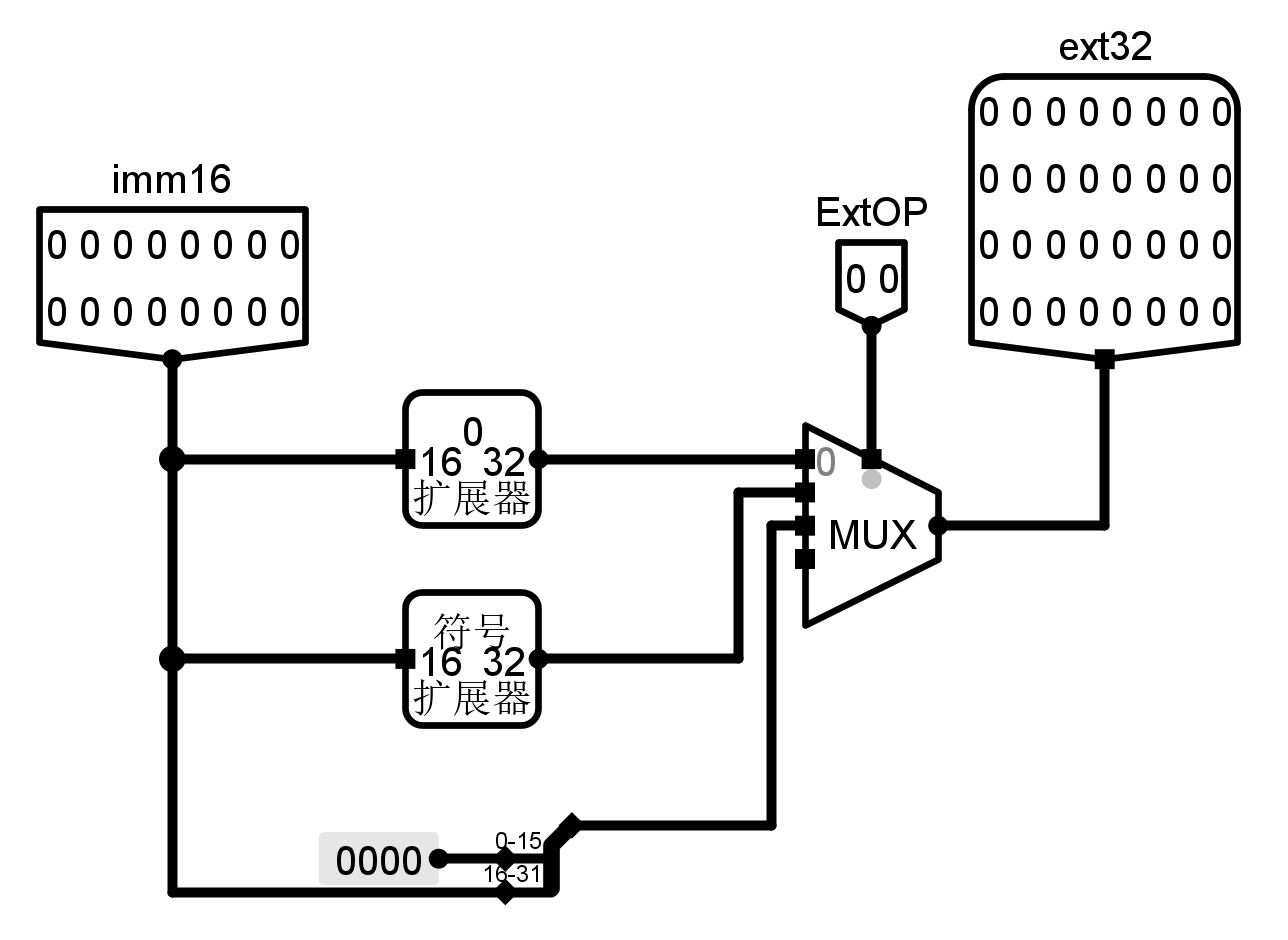
\includegraphics[width=\textwidth]{images/EXT-circuit.png}
\caption{EXT模块实现}
\end{figure}
EXT模块中,零拓展和符号拓展使用$LogicSim$内置的拓展器,而高位载入拓展使用一个分线器,高16位接入$imm16$,低16位接入常量$0x0000$。


\clearpage
\subsection{DM}
\subsubsection{基本描述}
DM作为系统主存,完成主存的读取和写入功能。
\paragraph{主存的读取}
根据输入的地址$addr$,输出对应的数据到$D_{out}$。
\paragraph{主存的写入}
根据输入的地址$addr$,将输入的数据$D_{in}$写入到对应位置。

\subsubsection{模块接口}
\begin{center}
    \captionof{table}{DM模块接口}
    \begin{tabular}[]{c c c l}
        \toprule
        信号名称 & 方向 & 位宽 & 描述 \\
        \midrule
        $clk$ & input & 1bit & 时钟信号。\\
        $clr$ & input & 1bit & \makecell[lt]{
            复位清空信号。\\
             0:复位。\\
             1:无效。
        } \\
        $WE$ & input & 1bit & 高有效写使能信号。\\
        $addrError$ & output & 1bit & \makecell[lt]{
            标明是否出现地址未对齐4的倍数。\\
             0:对齐4的倍数,正常。 \\
             1:未对齐4的倍数,出现错误。
        } \\
        \midrule
        $addr$ & input & 32bit & 读出或写入内存的地址。\\
        $D_{in}$ & input & 32bit & 写入的数据。 \\
        $D_{out}$ & output & 32bit & 读出的数据。\\
        \bottomrule
    \end{tabular}
\end{center}

\subsubsection{功能定义}
\begin{center}
    \captionof{table}{DM功能定义}
    \begin{tabular}{c c l}
        \toprule
        序号 & 功能名称 & 功能描述 \\
        \midrule
        1 & 复位 & $clr \land clk\uparrow \Rightarrow  Mem[i] = 0x00000000, i=0, 1, \dots 1023 $ \\
        2 & 读取内存值 & $ D_{out} \leftarrow Mem[addr] $ \\
        3 & 写入内存值 & $ WE \land clk\uparrow \Rightarrow Mem[addr] \leftarrow D_{in}$ \\
        4 & 地址错误检测 & $addrError \leftarrow \left( addr_{1..0} \neq 0b00 \right)$ \\
        \bottomrule
    \end{tabular}
\end{center}

\subsubsection{模块实现}
\begin{figure}[h]
\centering
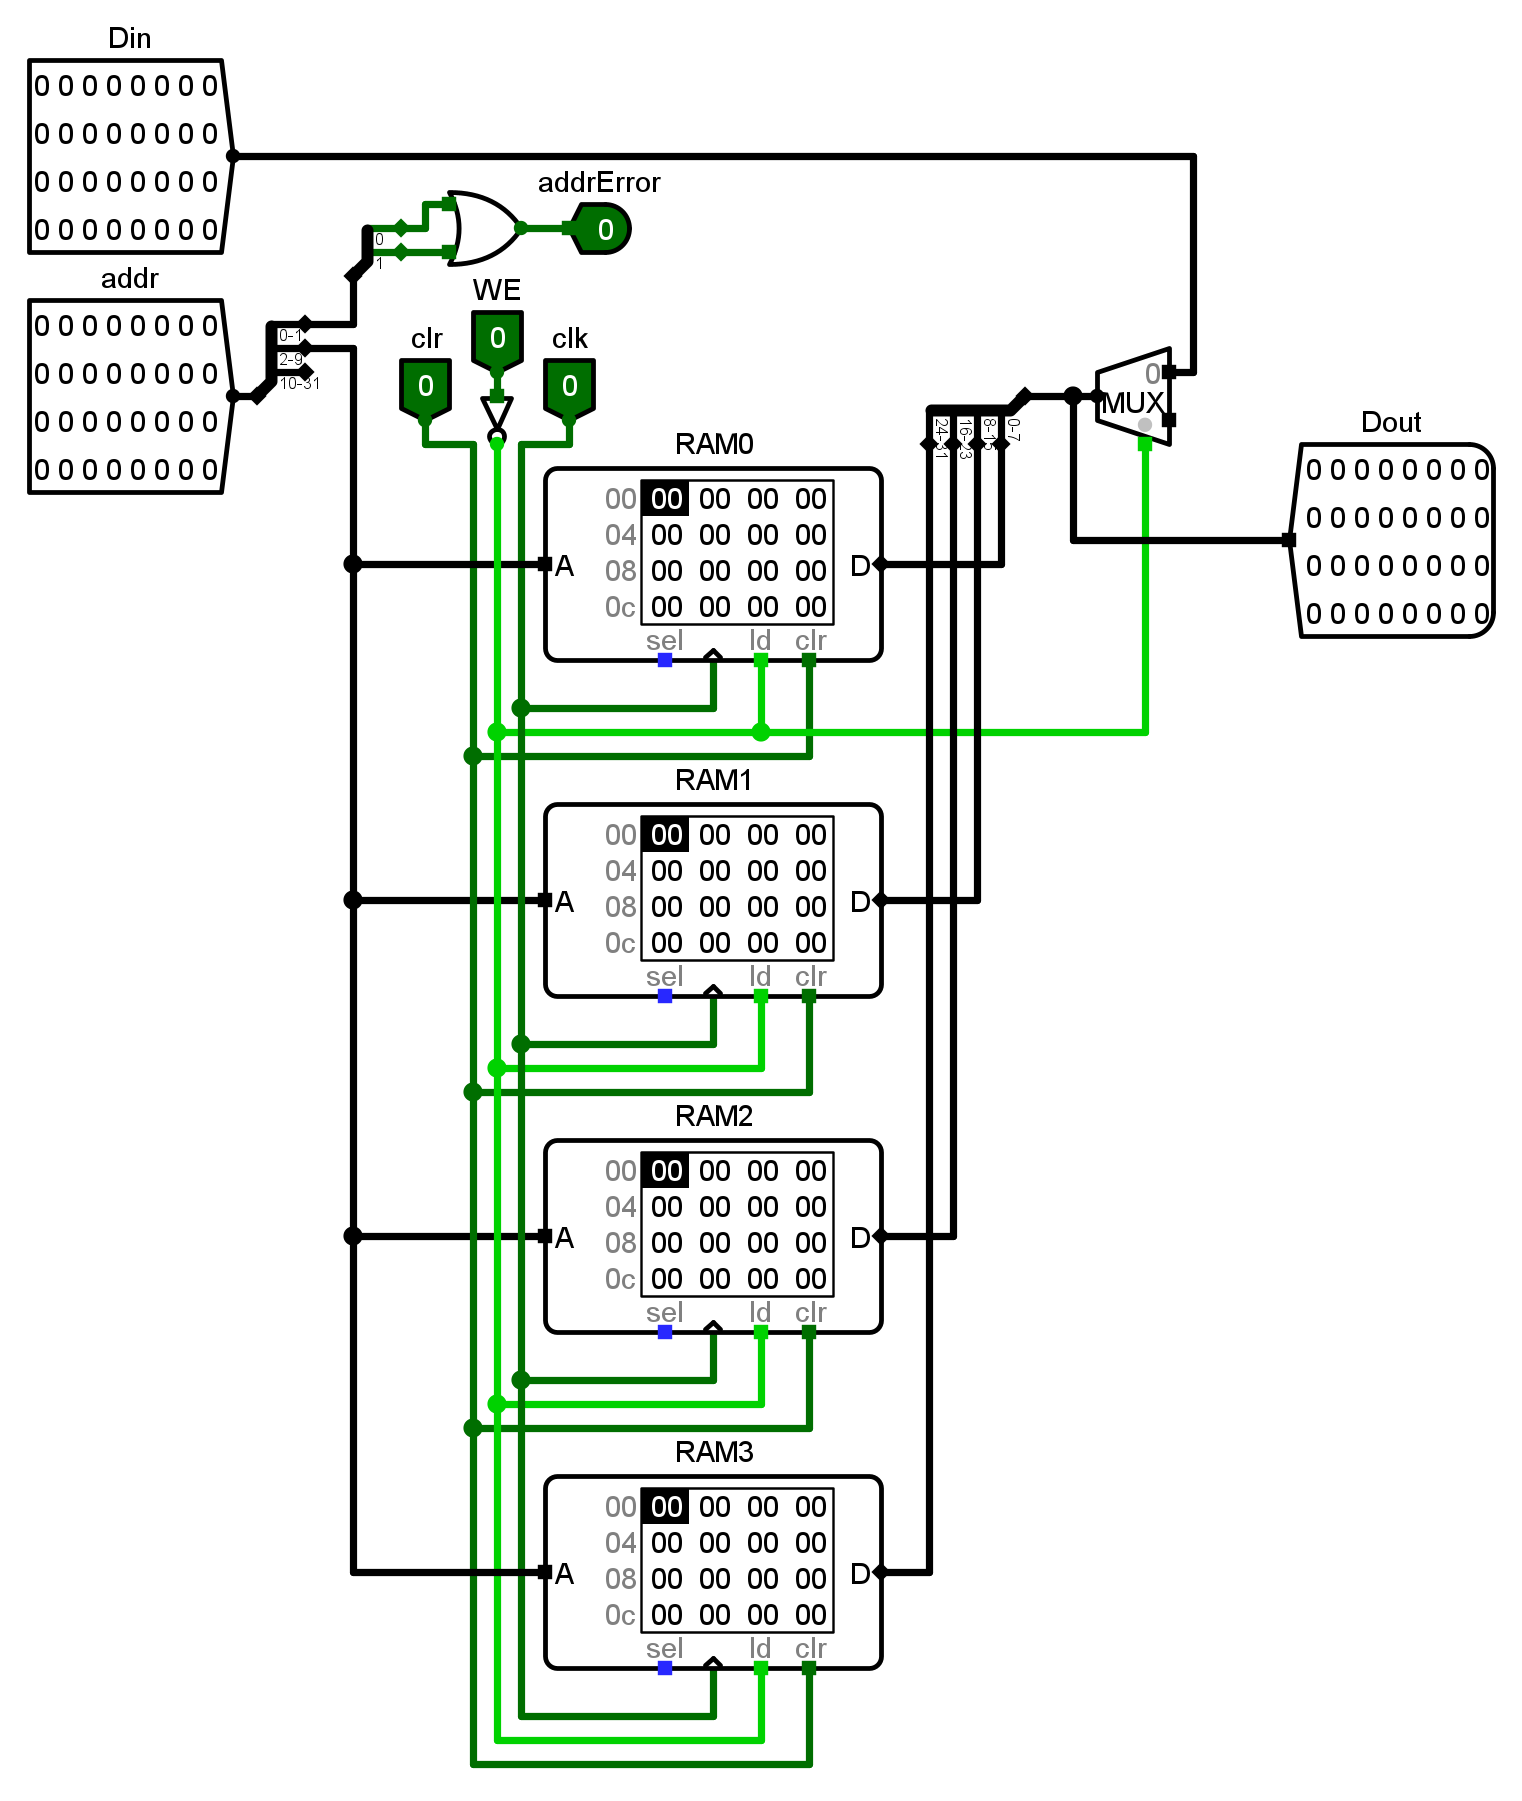
\includegraphics[width=\textwidth]{images/DM-circuit.png}
\caption{DM模块实现}
\end{figure}
$DM$内的数据存储由四个并行、小端序排列的$RAM$元件实现。

地址和控制信号$addr$、$clk$、$clr$、$WE$分别连接到四个$RAM$元件的$A$、$clk$、$clr$、$ld$端口。

数据方面,一个分线器将四个8位$RAM$元件和32位数据对应起来,使用小端序的形式(低位对应编号小的$RAM$,高位对应编号大的$RAM$)。所有时刻$D_{out}$与$RAM$的数据端$D$相连,而写入时$D_{in}$与$RAM$的数据端相连。

\end{document}
